\errorcontextlines9999
\documentclass[a3paper, portrait, english, default]{uulm-cs-poster}

\usepackage{lipsum}
\usepackage{wrapfig}
\usepackage{subcaption}
\usepackage{graphicx}
\graphicspath{ {./Bilder/} }

\title{flowR}
\subtitle{Layout Preserving Reconstruction}
\author{Pascal Deusch\and Florian Sihler}
\institute{Institut für Software Engineering und Programmiersprachen}
\university{Universität Ulm}
\logo{\splogo}
\date{\today}

\addbibresource{references.bib}
\nocite{*}

\begin{document}
\maketitle
%\section*{Why dogs are better cats}
%\lipsum[2]
%\vfil
\begin{multicols}{2}
\section*{FlowR}
   %Describtion of FlowR
	flowR is a static dataflow analyzer and program slicer for the R programming language.\\%reference flowR repo
	flowR allows its users to look at dataflow graphs for their R programs, generate slices for specified variables, and reconstruct those slices, amongst other functionalities.
	flowR is build in modules with its main modules being:
   \begin{itemize}
      \item a statistics module
      \item a benchmark module
	  \item a core module
      \item and a slicer module.
   \end{itemize}
The statistics module is used to analyze R files and identify common patterns in them. The benchmarker module serves as a way to benchmark flowR's performance.
The core module contains flowR's main definitions and is the home of flowR's read-eval-print loop (REPL) and flowR's server. The slicer module contains flowR's backward program slicer for R. This module consists of four submodules with a custom R bridge, a way to normalize the AST representation of the dataflow graph, a dataflow analyzer for said dataflow graph, and the reconstruct module.
My project is focused on the reconstruction module. There the work was mostly centered around the implementation of a layout-preserving reconstruction.
\paragraph{Reconstruction}
The reconstruction works in simple steps. The R parser parses the R code into an AST, which then gets normalized. This normalized AST is then traversed through a fold where the lexemes get put together with location information and additional tokens to create code parts. The code parts will, in a final step, get sorted and put together to form the final output.\\
Currently, the reconstruction can generate a layout-preserving reconstruction using the location information and additional tokens, however, not all additional tokens are currently in use. Mostly parentheses are being used to preserve the layout of loops. This, however, will be expanded in future updates to flowR, to iron out some quirks of the layout preserving reconstruction and possibly include the option for amorphous slicing.\\
\columnbreak
\section*{Layout Preserving Reconstruction}
	\begin{wrapfigure}{i}{0.2\textwidth}
		\begin{subfigure}[b]{0.2\textwidth}
			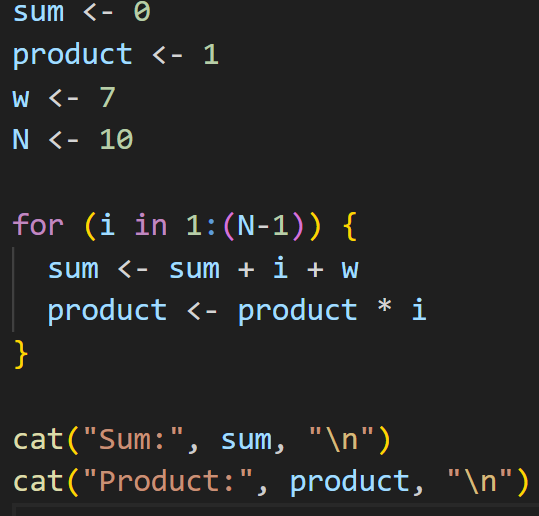
\includegraphics[scale=0.9]{Screenshot 2024-01-26 131317.png}
			\caption{Original R source code}
			\label{Fig.1}
		\end{subfigure}
		\begin{subfigure}[b]{0.2\textwidth}
			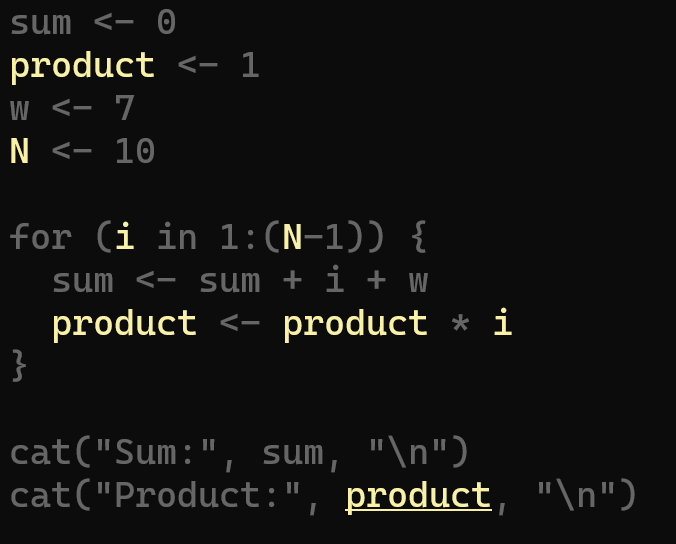
\includegraphics[scale=0.7]{Screenshot 2024-01-30 142858.png}
			\caption{Original R source code with sliced tokens highlighted}
			\label{Fig.2}
		\end{subfigure}
		\begin{subfigure}[b]{0.2\textwidth}
			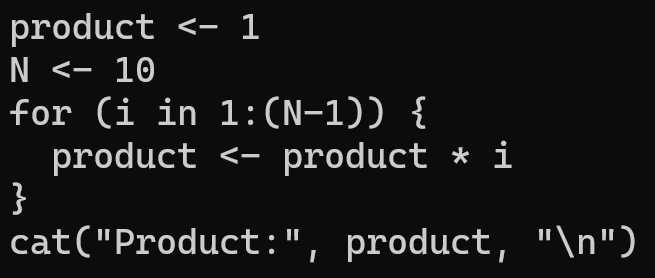
\includegraphics[scale=0.7]{Screenshot 2024-01-26 132150.png}
			\caption{Reconstructed slice for product in line 12}
			\label{Fig.3}
		\end{subfigure}
	\end{wrapfigure}
	The pictures on the left show an example of the reconstruction. The specific challenge in this case, was the reconstruction of the for-loop. The parser can differentiate between the single elements, however the implementation of the reconstruction had to be reworked significantly to use them. THe first step was to take the single elements the parser gave us and store them together with their location data. Those elements (parts) would then be stored in a monad imetating structure. We had to include the additional tokens the parser returns as well, since the paratheses, brackets, or even the "in" would not be available otherwise. This means that the reconstruction of the for loop has to construct every part of it seperatly and feed it into our output. To accomplish this we needed to add a way to put together multiple parts in their correct order. This gets accomplished over a single function (merge), which first sorts all parts by line, and afterward puts them together with sorted lines. \\
Printing the output gave us another challenge, as we had to work on each line individualy. We needed to keep track of each line length to avoid unwanted spaces but also make sure that all parts would be traversed in order.
   %\lipsum[4-6]
   %\paragraph{Paragraph}\lipsum[7]
\end{multicols}
%\lipsum[2]
\section*{My Contributions}
\begin{multicols}{4}
   %\lipsum[2]
	During my project, I refactored the structure of the preexisting reconstruction implementation. This was done to increase the readability of the module, as well as improve the quality for future improvements. The main part of the project so far has, however, been spent on improving the reconstruction by implementing layout preserving reconstruction.
	To achieve this we introduced two new parts. First we utalized the location information of the R parser to give the lexemes a position within the final output. Using this we then build up the code representation of the slice using the location information by first sorting all parts into their correct order and then appending all part together.
	Secondly, we introduced and utalized additional tokens, which include parenthesies and other special characters. These additional tokens then get added into the part with their locations, to get sorted and added to the output.
   %\printbibliography
\end{multicols}
\end{document}